\chapter{De gekozen oplossing}
\label{De_gekozen_oplossing}
%%%%%%%%%%%%%%%%%%%%%%%%%%%%%%%%%%%%%%%%%%%%%%%%%%%%%%%%%%%%%%%%%%%%%%%%

Om een keuze te maken tussen Advantics en Zero-EV zijn beide modems onderzocht,
en is de beste optie gekozen, in dit hoofdstuk word die keuze gemaakt en
uitgelicht.

%%%%%%%%%%%%%%%%%%%%%%%%%%%%%%%%%%%%%%%%%%%%%%%%%%%%%%%%%%%%%%%%%%%%%%%%
\section{Welk modum}
%%%%%%%%%%%%%%%%%%%%%%%%%%%%%%%%%%%%%%%%%%%%%%%%%%%%%%%%%%%%%%%%%%%%%%%%

Om een goede keuze te maken tussen Advantics en Zero-EV zijn beide modems
onderzocht door de datasheets en alle eigenschappen van deze modems te
bekijken. Daar zijn voordelen en nadelen uitgekomen voor beide modems.

%%%%%%%%%%%%%%%%%%%%%%%%%%%%%%%%%%%%%%%%%%%%%%%%%%%%%%%%%%%%%%%%%%%%%%%%
\subsection{Advantics}
%%%%%%%%%%%%%%%%%%%%%%%%%%%%%%%%%%%%%%%%%%%%%%%%%%%%%%%%%%%%%%%%%%%%%%%%

De eerste periode was besteed aan het kijken naar de mogelijkheden van het
Advantics systeem. In figuur \ref{fig:advantics_overzicht} zie je een overzicht
van alle componenten van het Advantics systeem. Centraal staat de \ac{ecu} met
geïntegreerd modem. Deze \ac{ecu} zit is ook gelijk de contactor controller.

\begin{figure}[h]
    \centering
    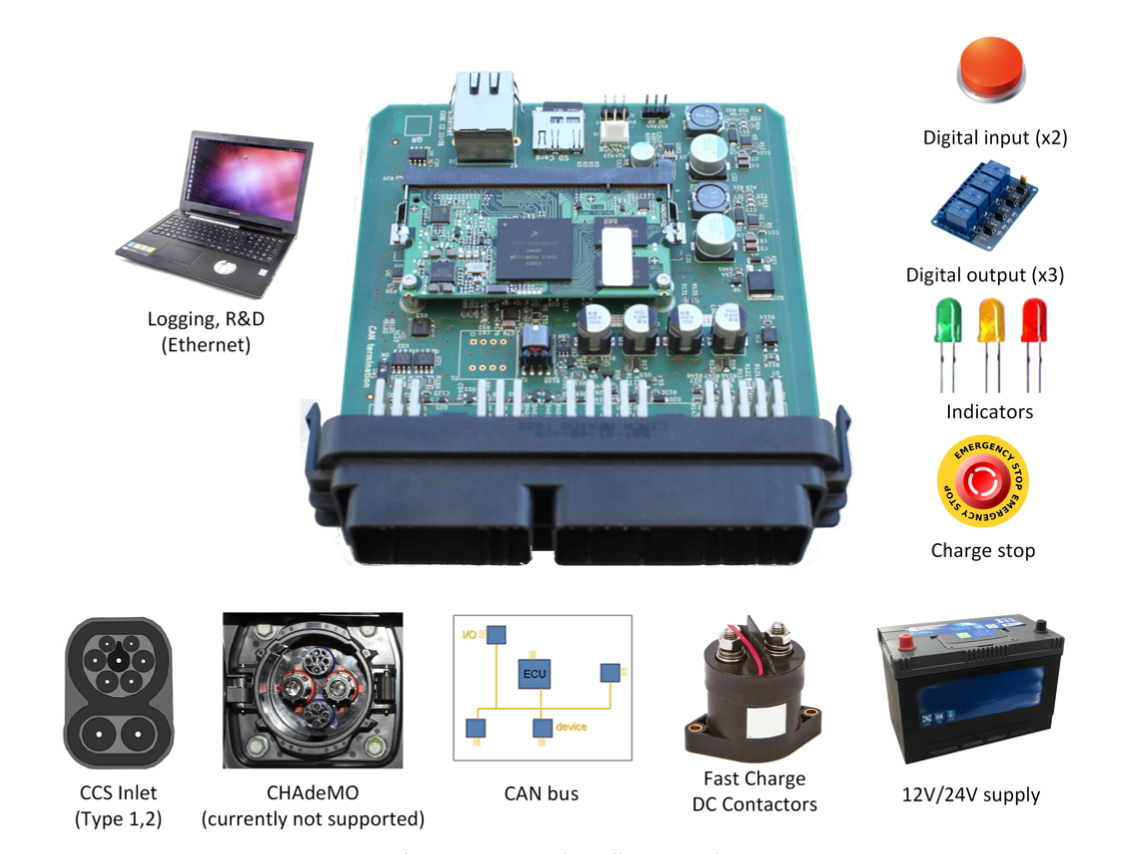
\includegraphics[width=0.85\textwidth]{advantics_overzicht}
    \caption{Overzicht van het Advantics systeem}
    \label{fig:advantics_overzicht}
\end{figure}

Waar al vrij snel tegen aan werd gelopen is dat de handleiding van dit systeem
incompleet is. Bovendien is de software die draait op de \ac{ecu} niet klaar om
te gebruiken. De fabrikant gaat ervan uit dat de gebruiker software schrijft
voor communicatie met het \ac{bms} en met de \ac{evse}. Maar het was niet
duidelijk hoe voor dit systeem ontwikkeld moest worden, als er geen/slechte
documentatie was.

\begin{table}[h]
    \begin{tabular}{|c|c|}
        \hline
        \multicolumn{2}{c}{Advantics} \\
        \hline
        Voordelen           & Nadelen \\
        \hline
        Heel erg uitgebreid & Moeilijk te gebruiken \\
        Veel mogelijkheden  & Er moet firmware voor ontwikkeld worden \\
        \hline
    \end{tabular}
\end{table}

%%%%%%%%%%%%%%%%%%%%%%%%%%%%%%%%%%%%%%%%%%%%%%%%%%%%%%%%%%%%%%%%%%%%%%%%
\subsection{Zero-EV}
%%%%%%%%%%%%%%%%%%%%%%%%%%%%%%%%%%%%%%%%%%%%%%%%%%%%%%%%%%%%%%%%%%%%%%%%

Hey systeem van Zero-EV zit iets anders in elkaar. Het systeem bestaat uit een
\ac{ecu} met een intern modem en een CCS contactor controller. Die onderdelen
communiceren met het BMS over de \ac{can} bus. In figuur
\ref{fig:zeroev_overzicht} zie je een overzicht van alle componenten van het
systeem.

\begin{figure}[h]
    \centering
    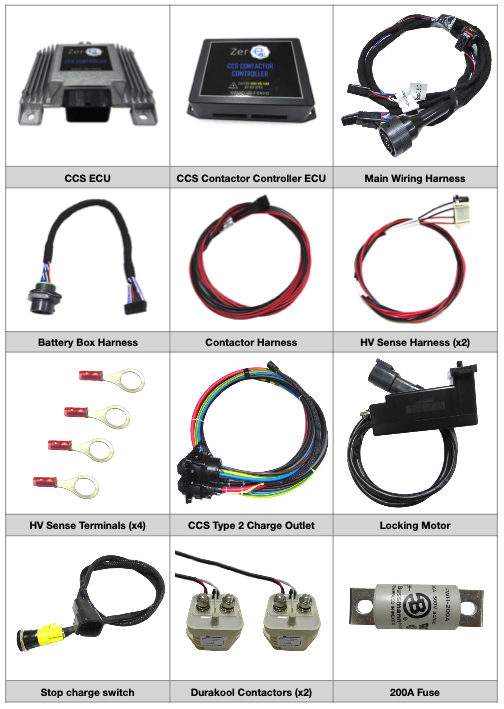
\includegraphics[width=0.45\textwidth]{zeroev_overzicht}
    \caption{Overzicht van het Zero-EV systeem}
    \label{fig:zeroev_overzicht}
\end{figure}

Het systeem van Zero-EV zou plug-and-play moeten zijn. Echter is dat alleen zo
als je een Orion BMS gebruikt, en EV Europe werkt met het EMUS BMS-systeem.

Als voor dit systeem wordt gekozen moet dus iets worden ontworpen dat er voor
zorgt dat het werkt met EMUS \ac{bms}.

\begin{table}[h]
    \begin{tabular}{|c|c|}
        \hline
        \multicolumn{2}{c}{Zero-EV} \\
        \hline
        Voordelen                          & Nadelen \\
        \hline
        Plug-and-play (met het juiste BMS) & Niet door de gebruiker te configureren \\
        Goede documentatie                 & \\
        \hline
    \end{tabular}
\end{table}

%%%%%%%%%%%%%%%%%%%%%%%%%%%%%%%%%%%%%%%%%%%%%%%%%%%%%%%%%%%%%%%%%%%%%%%%
\section{conclusie}
%%%%%%%%%%%%%%%%%%%%%%%%%%%%%%%%%%%%%%%%%%%%%%%%%%%%%%%%%%%%%%%%%%%%%%%%

Na tijd te hebben besteed aan beiden systemen, is in overleg met de
opdrachtgever er voor gekozen om verder te gaan met het systeem van Zero-EV.
Deze keuze is gebaseerd op de voordelen en nadelen van beide modems, en hoe
realistisch het is dat het systeem op tijd af is (binnen de stageperiode).
